\section{Circuiti RC e RL}

\begin{figure}[H]
    \centering
    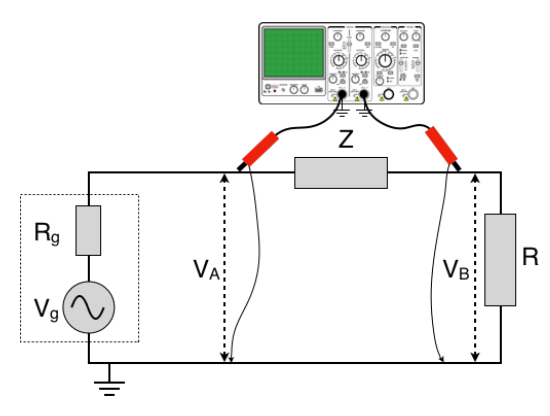
\includegraphics[scale=0.5]{Immagini/RC.PNG}
    \caption{}
\end{figure}


Per entrambe le configurazioni abbiamo disposto il circuito come in figura, dove Z indica rispettivamente il condensatore e l'induttore. Abbiamo, quindi, collegato le sonde come mostrato.
Grazie all'utilizzo dell'oscilloscopio abbiamo misurato diverse grandezze: le ampiezze $V_{A}$ e $V_{B}$ dei due segnali, l'ampiezza $V_{B-A}$ del sgnale differenza $V_{A}(t)$ - $V_{B}(t)$, la differenza di fase $\Delta \phi'$ tra il segnale di tensione ai capi di Z (tra $V_{A}(t)$ - $V_{B}(t)$ e $V_{A}(t)$) e la differenza di fase $\Delta \phi''$ tra $V_{A}(t)$ e $V_{B}(t)$.

Per ciascun circuito abbiamo riportato i dati in una tabella.

\subsection{Circuito RC}
Per svolgere la prima parte dell’esperienza abbiamo raccolto la maggior parte dei dati utilizzando i cursori dell’oscilloscopio, riportandoli successivamente nella seguente tabella; solo le differenze di fase sono state invece calcolate utilizzando i dati presi attraverso l'uso di una chiavetta USB

\begin{table}[!ht]
    \centering
    \begin{tabular}{lllll}
    \toprule
        $\nu$ [Hz]  & $\omega$ & $V_a$ [V] & $V_b$ [V] & $V_{a-b}$ [V]  \\ 
        \midrule
        25  & 3,98  & 2,48 & 0,32 & 2,48  \\ 
        35  & 5,57  & 2,18 & 0,38 & 2,16  \\ 
        45  & 7,16  & 1,92 & 0,42 & 1,88  \\ 
        60  & 9,55  & 1,62 & 0,44 & 1,56  \\ 
        80  & 12,73  & 1,36 & 0,48 & 1,24  \\ 
        90  & 14,32  & 1,24 & 0,5 & 1,16  \\ 
        100  & 15,92  & 3,76 & 1,56 & 3,44  \\ 
        200  & 31,83  & 2,48 & 1,68 & 1,84  \\ 
        300  & 47,75  & 2,21 & 1,68 & 1,28  \\ 
        \bottomrule
    \end{tabular}
    \caption{}
    \label{tabella 1}
\end{table}


Essendo la funzione di trasferimento un numero complesso abbiamo diviso il suo studio nell’analisi del modulo e nell’analisi della fase.
Riportiamo di seguito i moduli della funzione di trasferimento del circuito RC (in cui abbiamo 
usato R = 10$\Omega$), il primo utilizza la differenza di potenziale $V_{a}$ e $V_{b}$ e il secondo $V_{a-b}$ e $V_{b}$.

\begin{figure}[H]
    \centering
    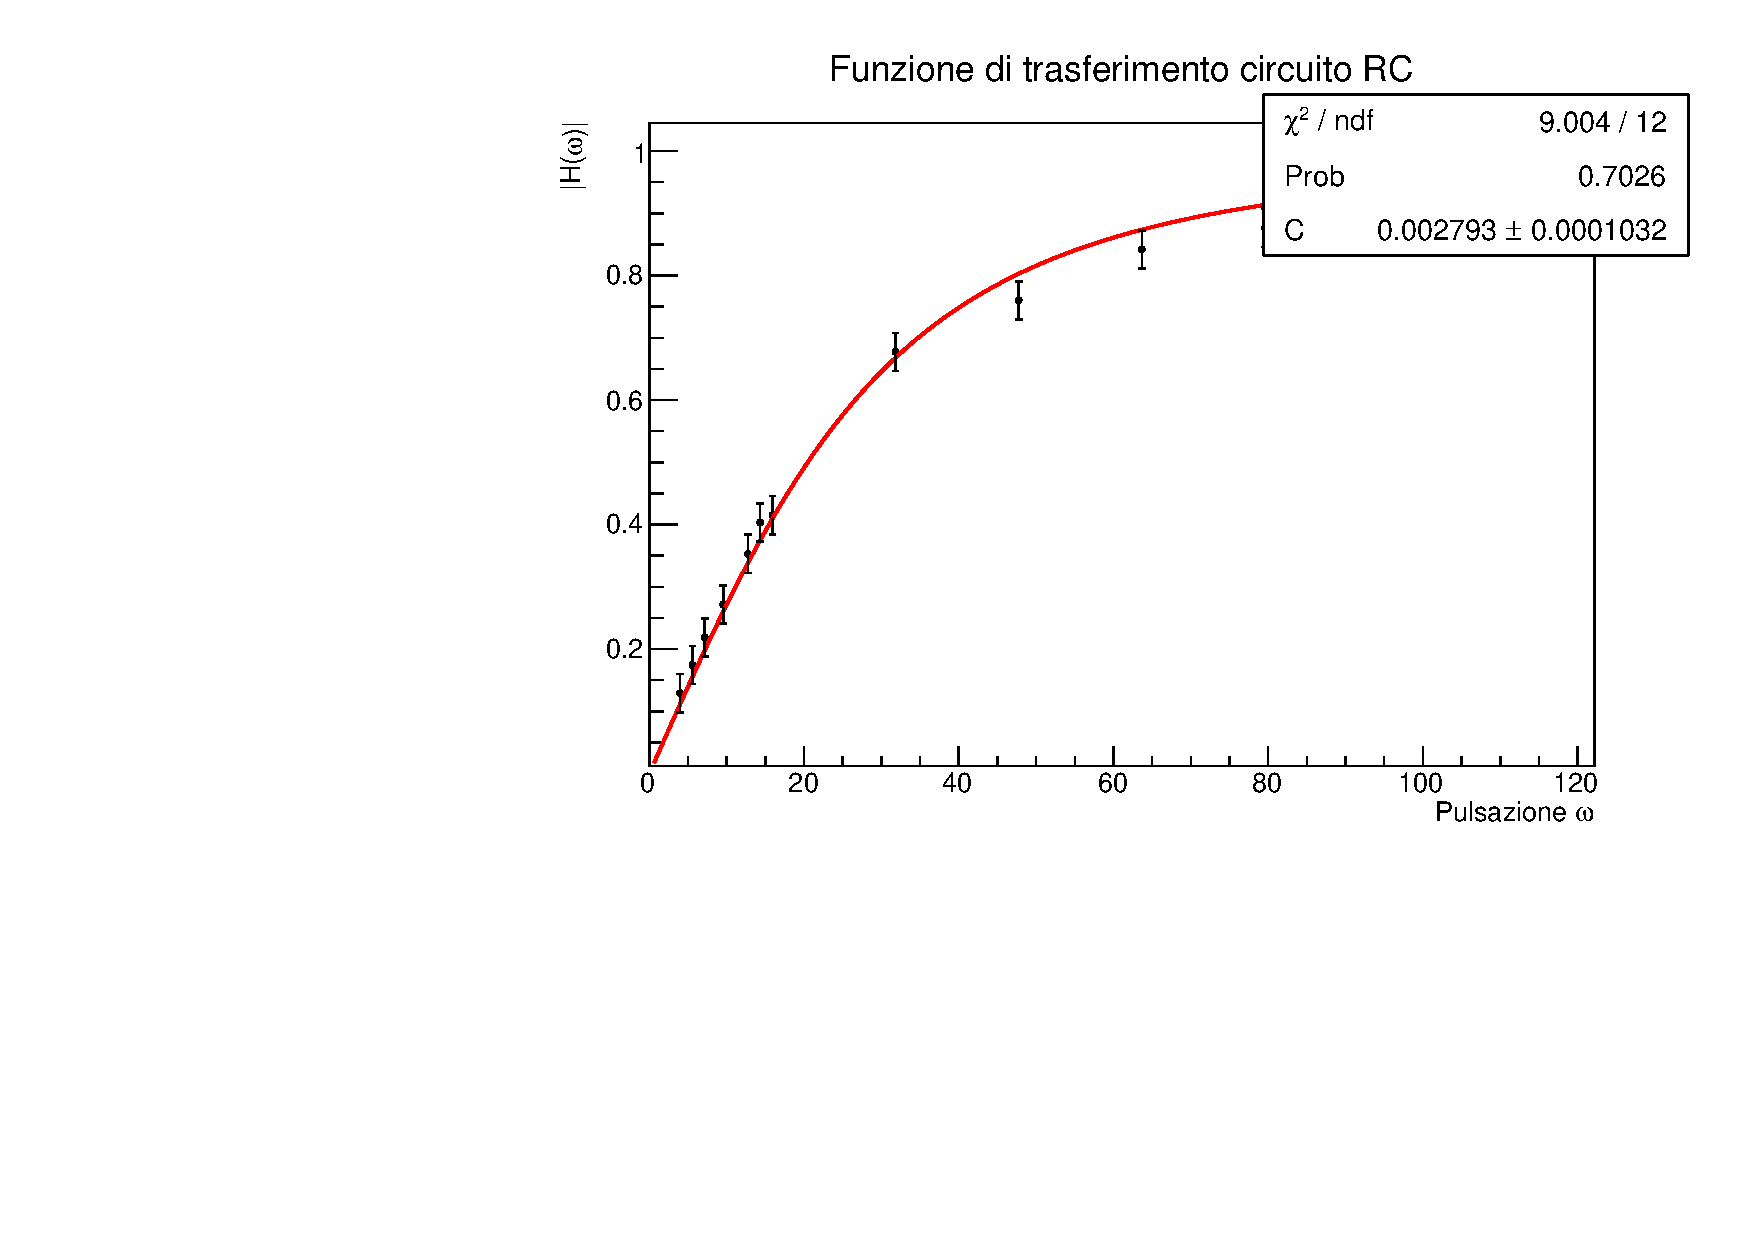
\includegraphics[scale=.4]{Immagini/trasferimento RC.pdf}
    \\
    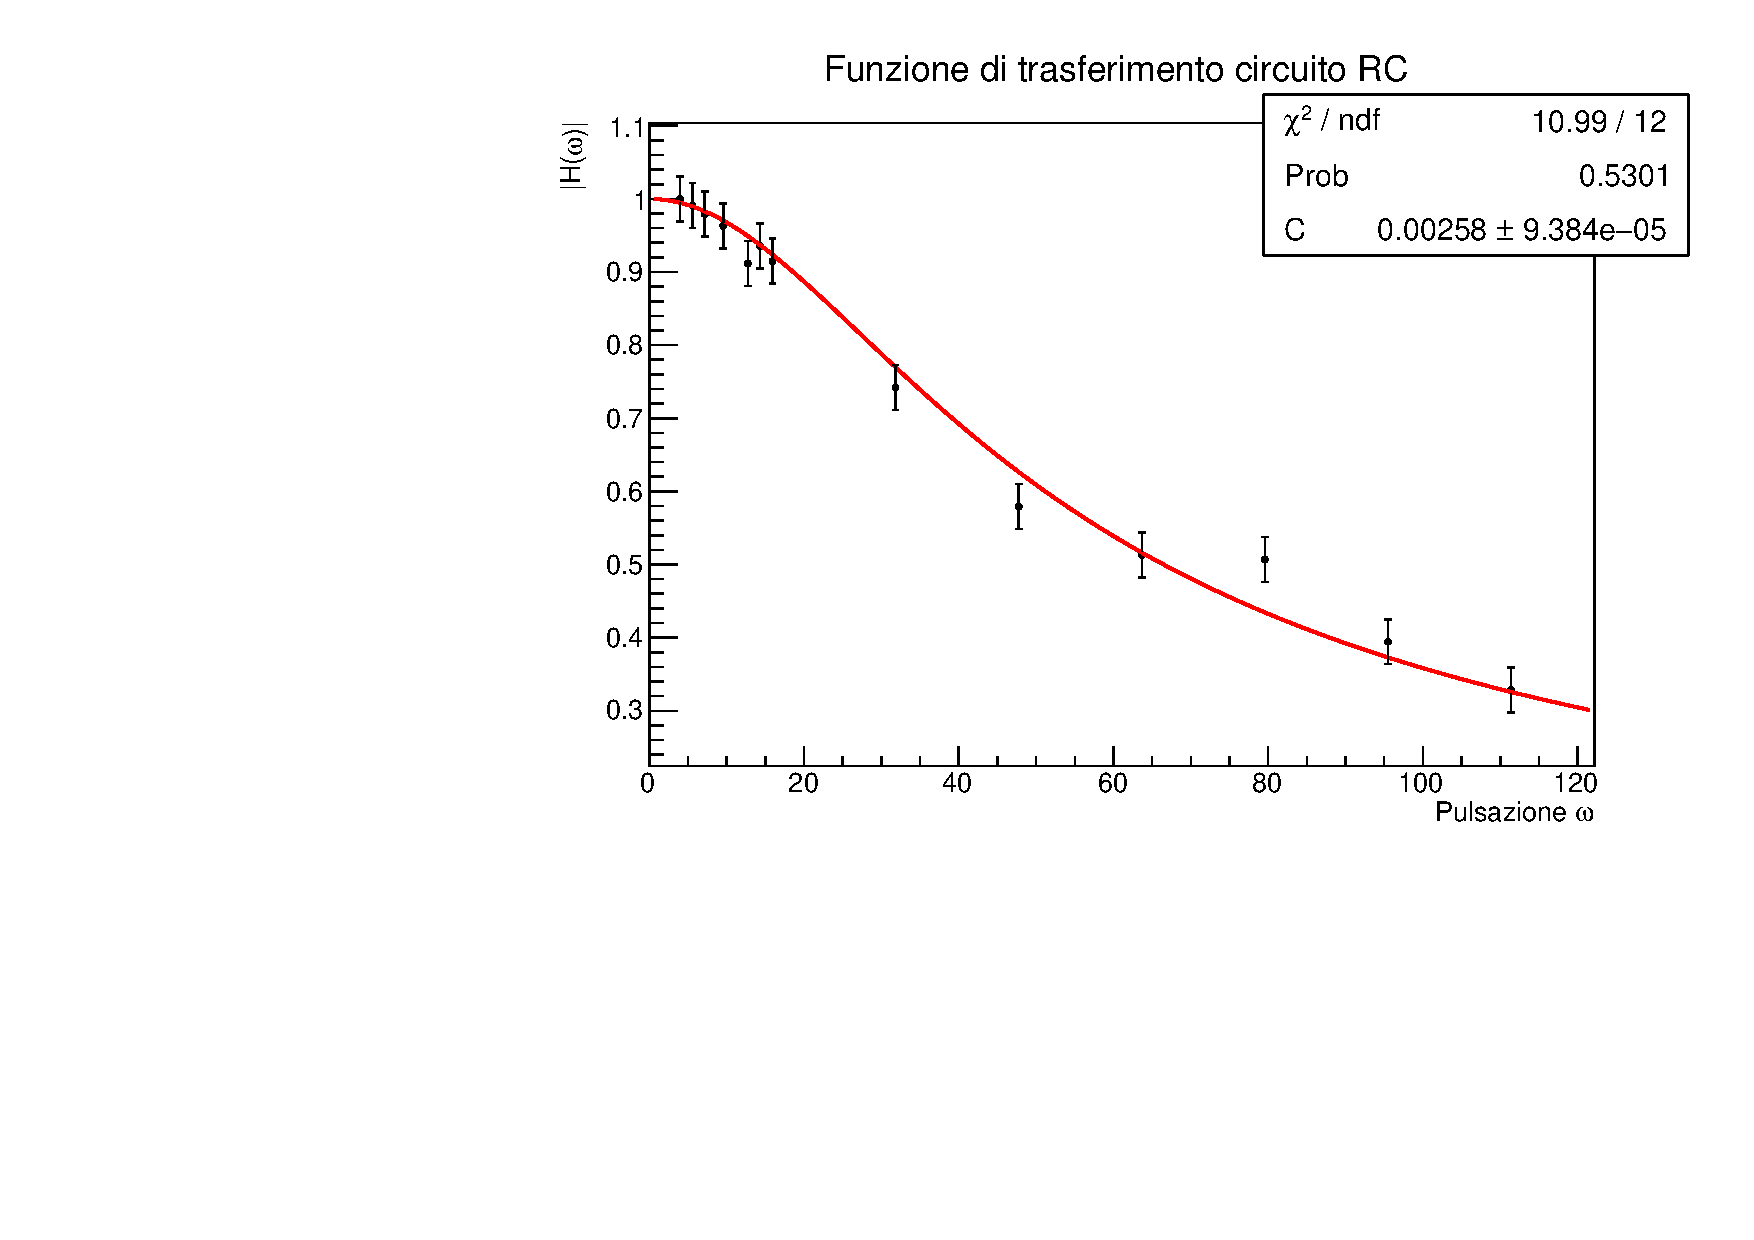
\includegraphics[scale=.4]{Immagini/trasferimento RC 2.pdf}
    \caption{}
\end{figure}

Il parametro \textit{C} corrisponde alla capacità, il suo valore è $(0,0027 \pm 0,0001) F$, inoltre il $\chi ^{2}$ accettabile conferma la relazione aspettata dal modello. Il valore ricavato della capacità è stato ricavato tramite una media pesata con la probabilità di $\chi^2$ dei due valori ricavati dal fit.
La scelta di \textit{R} per costruire il circuito è stata fatta in modo da avere una resistenza \textit{R} molto minore rispetto a quella interna dell’oscilloscopio.


\begin{figure}[H]
    \centering
    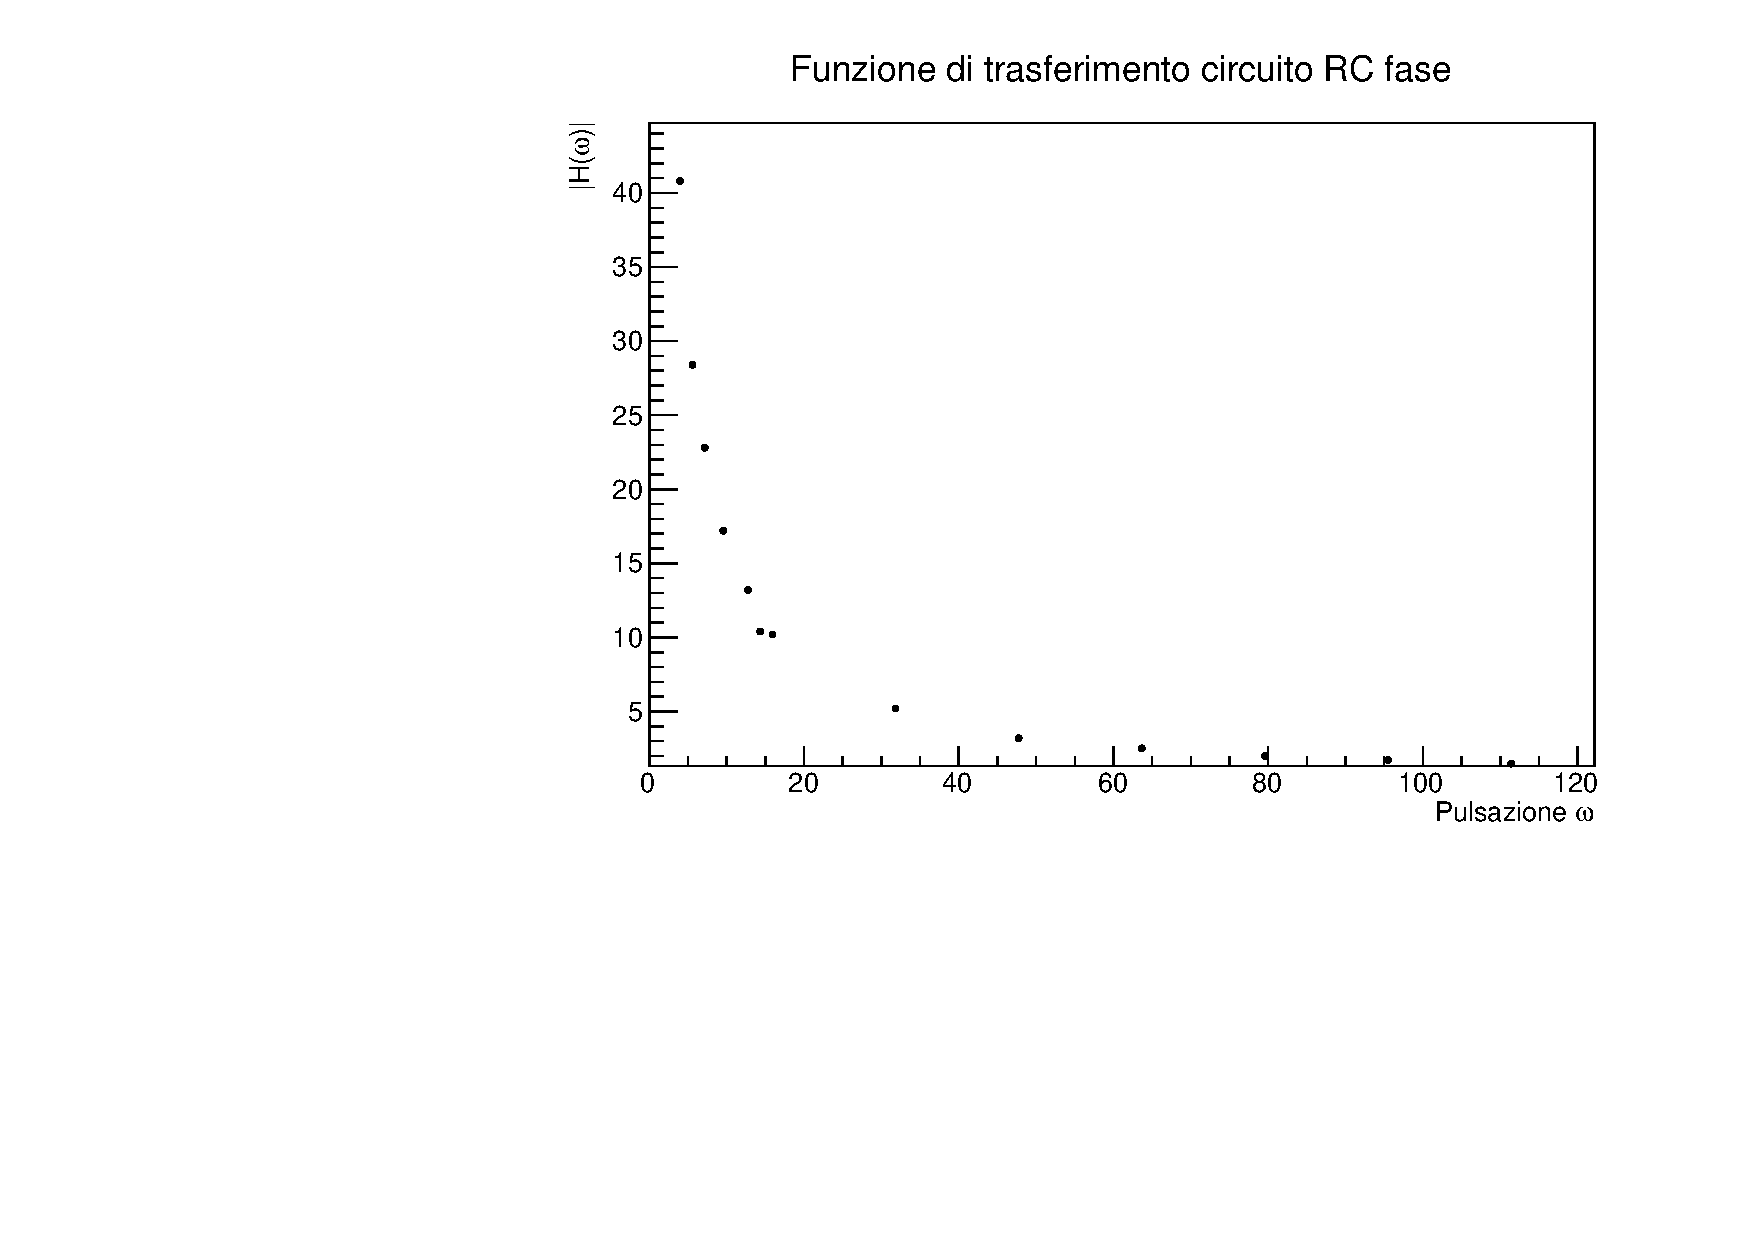
\includegraphics[scale=.4]{Immagini/fase RC.pdf}
    \caption{}
\end{figure}

Come si puo’ evincere dal grafico proposto, i dati raccolti non corrispondono al modello, che dovrebbe seguire un andamento arcotangente.
Le differenze di fase sono state calcolate come differenza 
tra gli zeri per assicurarci miglior precisione. Gli zeri sono stati ottenuti direttamente dall’oscilloscopio attraverso l'uso di una chiavetta USB, in modo tale da poter analizzare un range di 
dati legato alla precisione dello strumento stesso al posto che uno solo. Nonostante i nostri sforzi nel cercare di legare i dati al modello non siamo riusciti nell'intento. Abbiamo ipotizzato che le scale dei tempi fossero sbagliate, abbiamo tentato di calcolare le fasi attraverso le differenze di massimi e di minimi o interpolando l'intero andamento dei segnali per ricavare come parametro le varie fasi, abbiamo provato a lavorare con il modulo della differenza e abbiamo provato ridefinendo la funzione argomento. Nonostante tali accorgimenti non siamo riusciti a individuare una causa di errore attribuibile alla disposizione dei nostri dati rispetto al modello. Tenendo conto delle osservazioni qui riportate siamo costretti a dichiarare il nostro studio sulle fasi invalido.

\subsection{Circuito RL}
Similmente al circuito RC, nel caso di RL (in cui abbiamo utilizzato R = 1k$\Omega $) i moduli della fase di riferimento escono congruenti alla relazione descritta all’interno del modello.
\begin{table}[!ht]
    \centering
    \begin{tabular}{lllll}
    \toprule
        $\nu$ [Hz]  & $\omega$ & $V_a$ [V] & $V_b$ [V] & $V_{a-b}$ [V]  \\ \midrule
        20  & 3,18 & 2,94 & 2,78 & 0,24  \\ 
        50  & 7,96 & 2,94 & 2,76 & 0,28  \\ 
        100  & 15,91 & 2,96 & 2,76 & 0,32  \\
        300  & 47,75 & 2,96 & 2,76 & 0,56  \\
        500  & 79,57 & 3 & 2,72 & 0,88  \\ 
        800  & 127,32 & 2,96 & 2,6 & 1,2  \\ 
        1000  & 159,15 & 2,96 & 2,52 & 1,44  \\ 
        5000  & 795,77 & 3,08 & 1,16 & 2,88  \\
        10000  & 1591,54 & 3,04 & 0,68 & 3,12  \\ \bottomrule
    \end{tabular}
    \label{tabella 2}
    \caption{}
\end{table}

\begin{figure}[H]
    \centering
    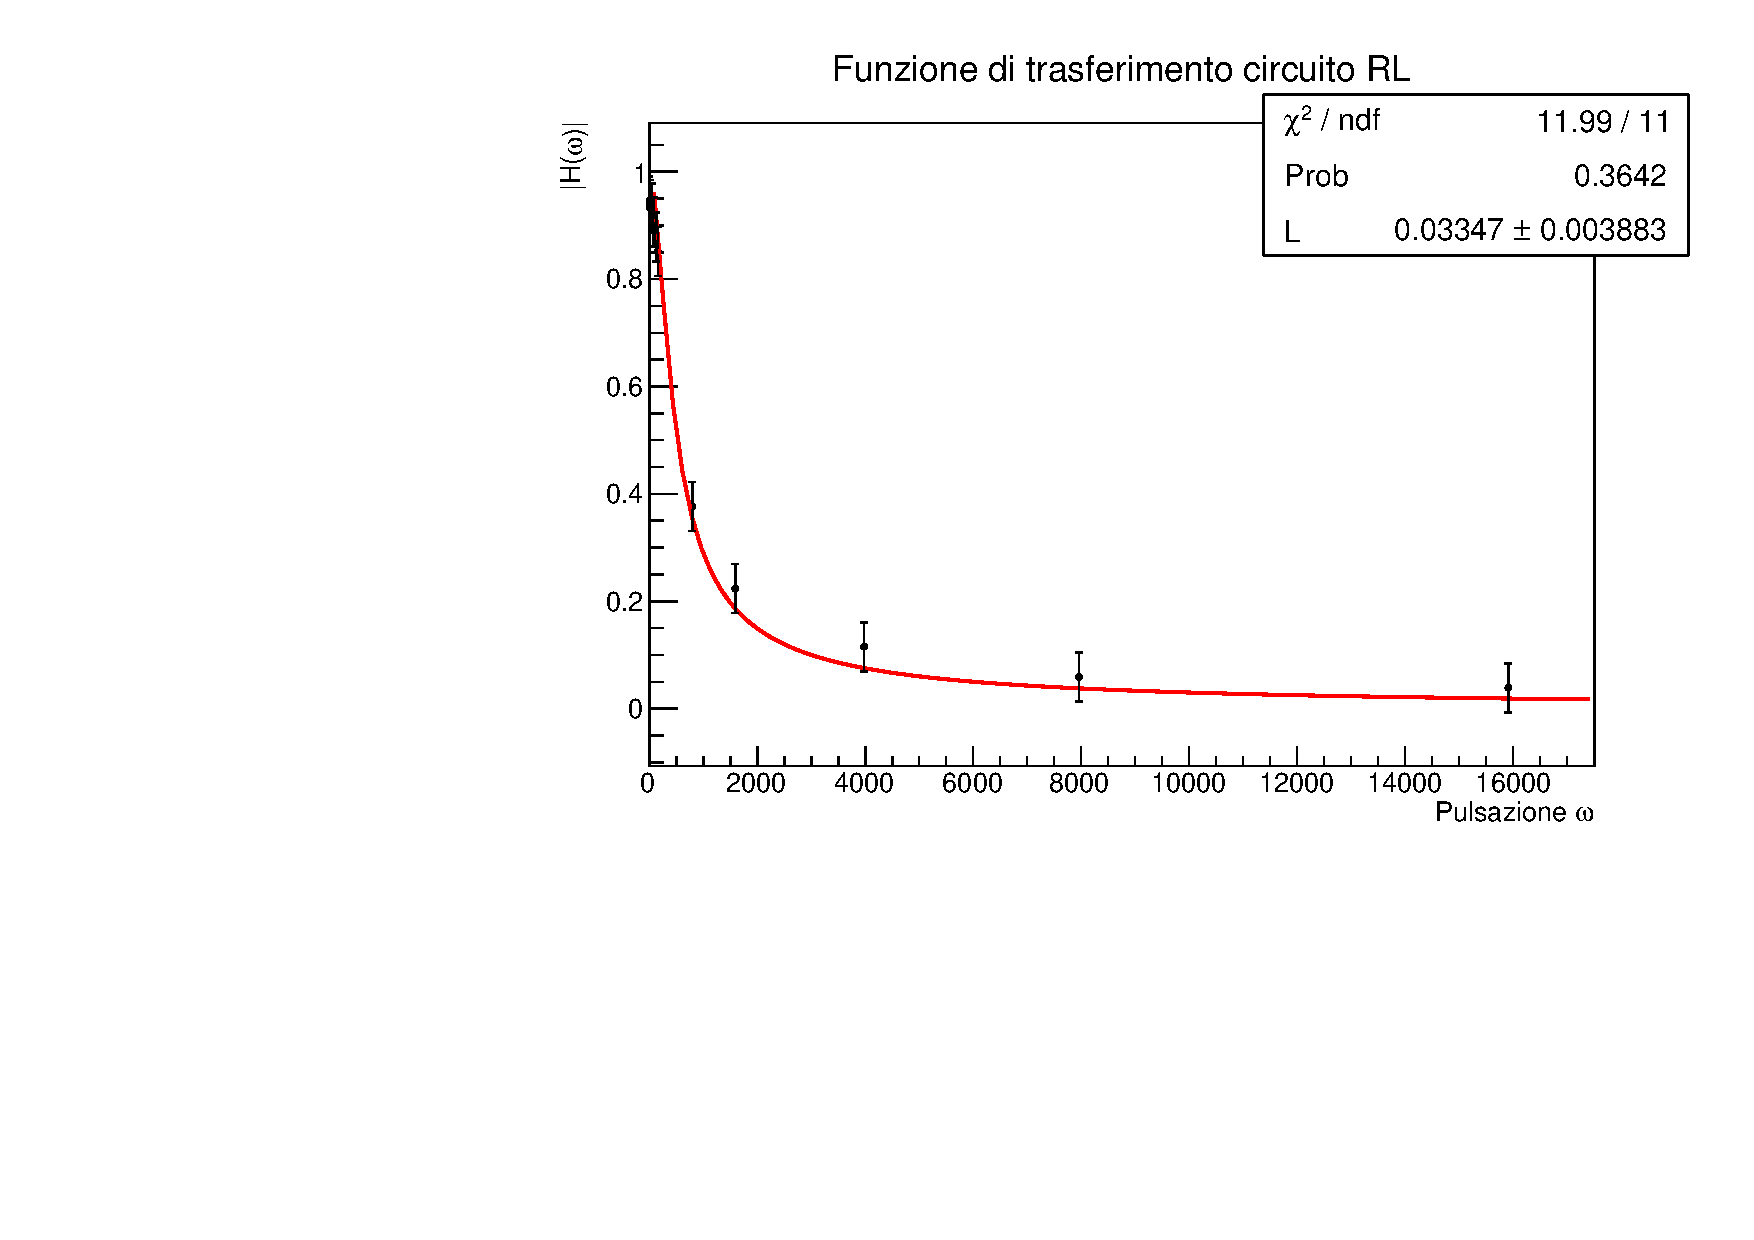
\includegraphics[scale=.4]{Immagini/trasferimento RL.pdf}
    \\
    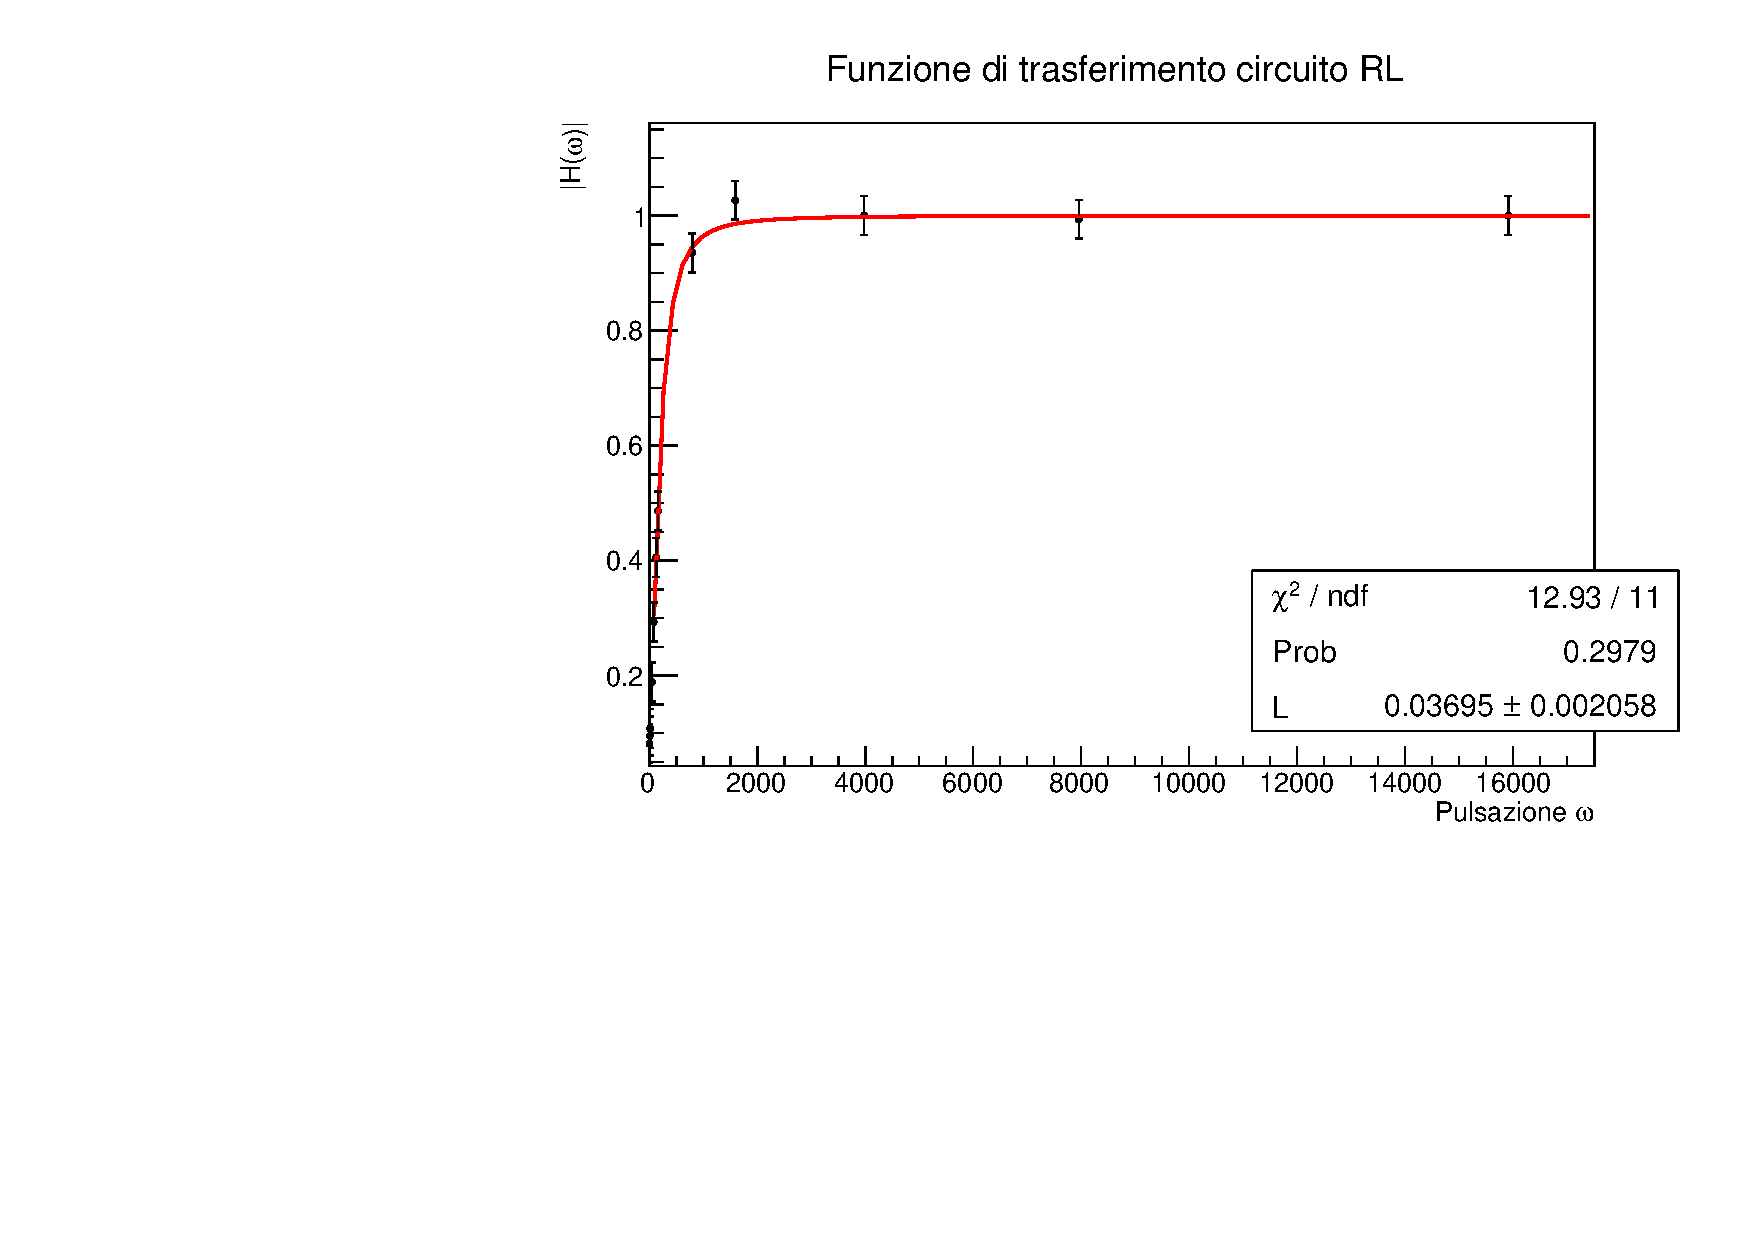
\includegraphics[scale=.4]{Immagini/trasferimento RL 2.pdf}
    \caption{}
\end{figure}

Abbiamo ricavato il valore di $\textit{L}=(0,0346 \pm 0,0001)H$, che corrisponde all’induttanza, ma per le fasi siamo incappati nello stesso problema che avevamo riscontrato per il circuito RC e che rende invalido  il nostro studio delle fasi. 
Il valore di L risulta accettabile in quanto nell’ordine della decina di \textit{mH}.
